\chapter{Technical Background}

\section{BERT}

As discussed in section \ref{sec:LR_NLP}, BERT is a transformer-based NLP model developed by Google that achieved state-of-the-art results in numerous NLP tasks when it was published in 2018 \cite{Devlin2018_BERT}.

\subsection{Architecture}

The architecture of the BERT model is based around that of a transformer, a type of deep learning model that tries to simulate the human process of attention by assigning different weights to the tokens in a given input sample based on their apparent relevance \cite{Bahdanau2014_Attention} \cite{sabharwal2021bert}.

Textual inputs passed into BERT are tokenised and segmented, with each part of the input being represented as a function of its token, its segment and its position. A diagram illustrating this representation, taken from \cite{Devlin2018_BERT}, can be seen in Figure \ref{fig:Explain_BERTEmbeddings}. This method of representation allows the model to consider the context of each particular token with regard to the tokens that come before and after it \cite{sabharwal2021bert}.

\begin{figure}[ht]
    \centering
    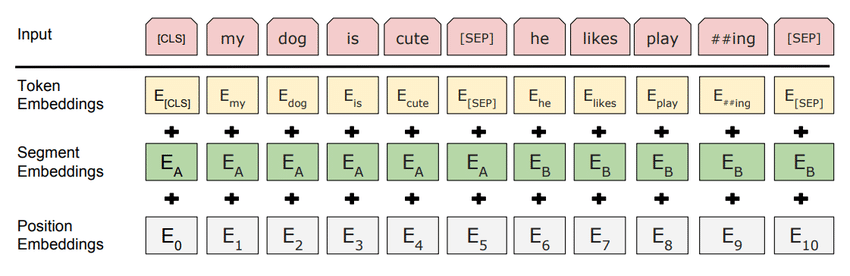
\includegraphics[scale=0.5]{figures/99_explanations/02_BERTEmbeddings.png}
    \caption{BERT input representation \cite{Devlin2018_BERT}.}
    \label{fig:Explain_BERTEmbeddings}
\end{figure}

These inputs are then fed through multiple encoding layers which try to determine how relevant different parts of the input are to each other through the aforementioned mechanism of attention \cite{AlammarTransformer}. The outputs from the encoding layer are passed through decoding layers before being passed through a softmax function to determine the final output \cite{Devlin2018_BERT}.

\subsection{Training}

The base BERT model was trained on over 3 billion words of data taken from English Wikipedia and BooksCorpus. The training process involved the completion of two tasks: masked language modelling and next sentence prediction. This initial training process is very time-consuming, generally taking multiple days to complete when using distributed cloud TPUs; although significant optimisations have been found that can reduce this time \cite{you2019large}.

\subsubsection{Masked Language Modelling}

This task involved the prediction of `masked' tokens in a sentence. Approximately 15\% of tokens in the dataset were replaced with \texttt{[MASK]} and the model's goal was to replace the masked tokens with the original terms \cite{Devlin2018_BERT}. For example, given the sentence ``I walked my \texttt{[MASK]} this morning'' as input, the model should produce the sentence ``I walked my dog this morning'' as output.

\subsubsection{Next Sentence Prediction}

This task involved the determination of whether or not two sentences ought to follow each other. The model would be given an initial sentence, \texttt{A}, and then given a second sentence, \texttt{B}, which, 50\% of the time directly followed \texttt{A} in the actual dataset and 50\% of the time was picked completely at random. The model's goal was to determine whether or not \texttt{B} actually followed \texttt{A} \cite{Devlin2018_BERT}. For example, given the sentences \texttt{A} = ``I walked my dog this morning'' and \texttt{B} = ``this is an unrelated sentence'', the model should determine that \texttt{B} does not follow \texttt{A}.

\subsection{Fine-tuning}

The fine-tuning process involves training the base BERT model on a smaller, specialised dataset, such as a collection of Steam reviews. This procedure is far less time-consuming than the initial training process and allows BERT to be quickly adapted to any NLP task \cite{Devlin2018_BERT}.

\subsection{DistilBERT}

The DistilBERT model \cite{sanh2019distilbert} is a pre-trained language representation model that is based on BERT but has been reduced in size by 40\% through the process of knowledge distillation, a process that reduces the size of a machine learning model without diminishing its predictive validity \cite{hinton2015distilling}. The resulting model, according to the authors, is 60\% faster than BERT and ``retains 97\% of its language understanding capabilities''.

\subsection{Exact Models Used}

Two pre-trained DistilBERT models were used over the course of this project: \texttt{distilbert-base-uncased} \cite{HuggingFaceEng} for fine-tuning with English samples and \texttt{distilbert-base-multilingual-cased} \cite{HuggingFaceMulti} for fine-tuning with multilingual samples. Both of these models were taken from Hugging Face \cite{wolf2019huggingface}. 

\section{Text Processing}

\subsection{Preprocessing}

Text data is often preprocessed before it is fed into a model. This can involve the conversion of the text to lowercase, particularly when the text is written in English; the splitting of the sentence into tokens; the removal of stop words; and the construction of $n$-grams from the remaining tokens.

\subsubsection{Tokenisation}

Tokenisation is the process by which a sample of text is split into a list of its component words or tokens, this is usually done based on the presence of punctuation marks, eg periods or commas, and spaces.

\subsubsection{Stop words}

Stop words are a set of very common words in a language, such as `the' or `and' in English, that tend to be filtered out or ignored in the process of text processing. This is based on the assumption that they carry very little useful information regarding any particular sample of text. Different languages have different sets of stop words and there is no universally agreed upon list of stop words for any particular language.

\subsubsection{N-grams}

$N$-grams are sets of $n$ consecutive tokens taken from a sample of text. For example, the set of $n$-grams of length 2, called bigrams, in a sentence would consist of a tuple for each consecutive pair of words. $N$-grams of length 1 are called unigrams while $n$-grams of length 3 are called trigrams.

\subsubsection{Examples}

Some examples of the above processes are given in Table \ref{tab:Explain_TextProc}.

\begin{table}[ht]
    \centering
    \begin{tabular}{l l}
        \toprule
        \textbf{Process} & \textbf{Result} \\\midrule
        Original & `Be quiet, the baby is sleeping.'\\
        Lowercased & `be quiet, the baby is sleeping.'\\
        Tokenised & `be', `quiet', `the', `baby', `is', `sleeping'\\
        Stop words removed & `quiet', `baby', `sleeping'\\
        Unigrams & (`quiet'), (`baby'), (`sleeping')\\
        Bigrams & (`quiet baby'), (`baby sleeping')\\
        Trigrams & (`quiet baby sleeping')\\
        \bottomrule\\
    \end{tabular}
    \caption{Examples of text preprocessing techniques applied in succession.}
    \label{tab:Explain_TextProc}
\end{table}

\subsection{Vectorisation}

Once a sample of text has been preprocessed it can be vectorised, a process that involves the mapping of its tokens to numerical values.

\subsubsection{Bag-of-words}

A simple example of text vectorisation is the bag-of-words model which tracks the particular tokens that were present in a sample as well as the frequency with which each token occurred. It's worth noting that this vectorisation model disregards the order in which tokens occurred in the text; however, when the technique is applied to $n$-grams, certain word orderings can be somewhat preserved. The set of distinct tokens that occur in all of the text samples is called the vocabulary and each token in the vocabulary is also mapped to a numerical value beginning at 0 and counting up. An example of bag-of-words vectorisation is given in Table \ref{tab:Explain_BOW}.

\begin{table}[ht]
    \centering
    \begin{tabular}{l l}
        \toprule
        \textbf{Process} & \textbf{Result} \\\midrule
        Original & `Be quiet, the baby is sleeping. The dog is also sleeping.'\\
        Preprocessed (unigrams) & `quiet', `baby', `sleeping', `dog', `also' `sleeping'\\
        Vectorised & $\begin{bmatrix} \text{`quiet'} & 1\\ \text{`baby'} & 1\\ \text{`sleeping'} & 2\\ \text{`dog'} & 1\\ \text{`also'} & 1\\ \end{bmatrix} \longrightarrow \begin{bmatrix} 1&1&2&1&1\\ \end{bmatrix}$\\
        \bottomrule\\
    \end{tabular}
    \caption{Example of bag-of-words vectorisation applied to a sentence}
    \label{tab:Explain_BOW}
\end{table}

\subsubsection{TF-IDF}

TF-IDF is a statistic used to weight the vectorised term (token) counts in each sample according to the frequency with which the term in question occurs in all of the samples in the dataset. The weights are then normalised using the Euclidean norm. For a given text sample, $s$, and a particular term, $t$, in a dataset containing $n$ total samples, the formula for calculating the TF-IDF weighting, taken from the documentation for \cite{pedregosa2011scikit}, is as follows:

\begin{equation*}
    v_{t,s} = \mathrm{tf}(t, s) \left( \log{\frac{n}{\mathrm{df}(t)}} + 1 \right)
\end{equation*}

where $\mathrm{tf}(t, s)$ is the number of times $t$ occurred in $s$ and $\mathrm{df}(t)$ is the number of samples $t$ appeared in. The normalisation formula, again taken from the documentation, is as follows:

\begin{equation*}
    v_{t,s}' = \frac{v_{t,s}}{\sqrt{\sum_{i=0}^n v_{t,i}^2}}
\end{equation*}

\section{Feature Scaling}

Feature scaling is a technique in machine learning preprocessing in which the values of numerical features, which might span any range, are normalised to fit into a finite defined range such as $[0,1]$ or $[-1,1]$. A very simple scaling technique, referred to as min-max scaling in the \cite{pedregosa2011scikit} documentation, involves the mapping of a list of values into the range $[0,1]$ with the maximum original value becoming 1, the minimum original value becoming 0 and the remaining values falling somewhere in between.

\subsection{Robust Scaling}

For data containing extreme or outlier values, techniques such as min-max scaling can produce poor results as most normalised values will be very similar with only the outliers being close to 0 or 1. A simplified description of robust scaling is that it scales values according to the interquartile range, ie the difference between the values in the 75th and 25th percentiles, as opposed to the median or the minimum and maximum values \cite{pedregosa2011scikit}. This technique reduces the influence of outliers on the resulting normalised values.

\section{Machine Learning Models}

\subsection{Baseline Classifiers}

Baseline or `dummy' classifiers are often used in comparison to trained models to better evaluate the trained models' performance. A simple baseline classifier is one that always predicts the most common label in the training data. A uniformly random classifier would predict any one of the labels in the training data at random, with each label having the same likelihood of being predicted. A slightly more advanced random classifier, which is better suited to data with more than two labels, would predict any one of the labels in the training data at random, with label probabilities being proportional to how often they actually occur in the data \cite{pedregosa2011scikit}.

\subsection{Naive Bayes Classifiers}

NB classifiers utilise Bayes' theorem to make predictions based on conditional probability, eg the probability that a sample should be classified as positive given a certain input feature. The meaning of the term `naive' comes from the fact that, when determining an overall classification based on numerous input features, conditional independence is naively assumed to exist between each set of input features which vastly reduces the amount of time and memory required to carry out calculations \cite{dangeti2017statistics}. As a result, NB classifiers tend to be very efficient \cite{pedregosa2011scikit}.

\subsubsection{Multinomial Naive Bayes}

A multinomial naive Bayes (MNB) classifier is a type of NB classifier that is particularly suited to text classification due to its modelling of the frequencies of terms in a sample, and the entire dataset, as a multinomial \cite{rennie2003tackling}.

\subsubsection{Complement Naive Bayes}

A complement naive Bayes (CNB) classifier is an adapted version of the MNB classifier which is better suited towards imbalanced datasets due to the fact that it is trained using the complement of the desired class, ie the probability that the given sample is \textit{not} a member of the desired class \cite{pedregosa2011scikit} \cite{rennie2003tackling}.

\subsection{Support Vector Machines}

Support vector machines (SVM), specifically linear SVMs, are a group of machine learning models that can be used for both classification and regression. When trained for classification, linear SVMs attempt to find a linear separation between both classes in the training data, using a hyperplane, while also maximising the distance between training points on the separation boundaries and the hyperplane itself \cite{dangeti2017statistics}. When more than two classes are present a one-vs-rest strategy is used to break the classification problem down into multiple binary classification problems \cite{pedregosa2011scikit}. An illustration of an SVM classifier can be seen in Figure \ref{fig:Explain_LSVC}.

\begin{figure}[ht]
    \centering
    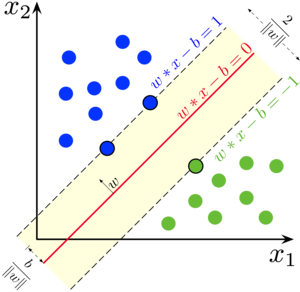
\includegraphics[scale=4]{figures/99_explanations/01_LSVC.png}
    \caption{Example of an optimal hyperplane found by an SVM classifier for two classes \cite{WikipediaLSVC}.}
    \label{fig:Explain_LSVC}
\end{figure}

When trained for regression, linear SVMs attempt to fit a hyperplane to the training data that contains the maximum number of data points \cite{smola2004tutorial}.

\subsubsection{Stochastic Gradient Descent}

Stochastic gradient descent (SGD) is an optimisation algorithm for minimising the cost function of a machine learning model, over numerous iterations, using approximations of the function's actual gradient calculated from multiple subsets of the training data. SGD is highly efficient and can be used for both classification and regression problems. SGD can be used in linear SVM classifiers and regressors \cite{pedregosa2011scikit}.

\subsection{Baselines Regressors}

As was the case with classifiers, baseline or `dummy' regressors are often used in comparison to trained models. Two simple examples of baseline regressors are those that always predict either the mean or the median of the values in the training data \cite{pedregosa2011scikit}.

\subsection{Ridge Regressors}

Ridge regression models use least squares regression combined with a regularisation penalty, which includes the sum of the squares of the regression coefficients in the cost function in order to reduce overfitting \cite{dangeti2017statistics}.

\section{Evaluation Metrics}

\subsection{Classification}

\subsubsection{True and Predicted Labels}

In a classification task involving two labels, positive and negative, predictions can be split into four categories depending on the true label and the predicted label of the item in question. These categories are shown in the confusion matrix in Table \ref{tab:Explain_ConfMat}.

\renewcommand\arraystretch{1.5}
\begin{table}[ht]
    \centering
    \begin{tabular}{l|l|c|c|}
        \multicolumn{2}{c}{} & \multicolumn{2}{c}{True}\\
        \cline{3-4}
        \multicolumn{2}{c|}{} & Positive & Negative\\
        \cline{2-4}
        \multirow{2}{*}{Predicted}& Positive & True positive (TP) & False positive (FP)\\
        \cline{2-4}
        & Negative & False negative (FN) & True negative (TN)\\
        \cline{2-4}
    \end{tabular}
    \caption{Confusion matrix for binary classification}
    \label{tab:Explain_ConfMat}
\end{table}

\subsubsection{Accuracy}

The accuracy of a classifier is the proportion of predicted labels that match the true labels:

\begin{equation*}
    \mathrm{Accuracy} = \frac{TP + TN}{TP + FP + TN + FN}
\end{equation*}

Accuracy can give a general overview of how well a classifier is performing but it can be a poor evaluation metric in datasets with an imbalanced number of positive and negative items.

\subsubsection{Precision and Recall}

The precision of a classifier is the ratio of true positive predictions to total positive predictions:

\begin{equation*}
    \mathrm{Precision} = \frac{TP}{TP + FP}
\end{equation*}

The recall of a classifier is the ratio of true positive predictions to total positive items:

\begin{equation*}
    \mathrm{Recall} = \frac{TP}{TP + FN}
\end{equation*}

Precision and recall, used in conjunction, can provide better insight into the predictive capability of a classifier, particularly when the dataset being used is imbalanced.

\subsubsection{$F_1$-score}

The $F_1$-score of a classifier is a measure of its overall accuracy using the harmonic mean of the precision and recall values:

\begin{equation*}
    F_1 = \frac{2 \cdot \mathrm{Precision} \cdot \mathrm{Recall}}{\mathrm{Precision} + \mathrm{Recall}}
\end{equation*}

The use of the harmonic mean of both values rather than the arithmetic mean ensures that higher $F_1$-scores, which indicate a better result, can only occur when both precision and the recall are high themselves.

\subsubsection{Receiver Operating Characteristic}

The receiver operating characteristic (ROC) curve compares the true positive rates (TPR) and false positive rates (FPR) of a classifier as its decision threshold is varied. The TPR is equivalent to the recall value while the FPR is the ratio of false positive predictions to total negative items:

\begin{equation*}
    \mathrm{FPR} = \frac{FP}{TN + FP}
\end{equation*}

The decision threshold of a classifier is the value at which a predicted probability score for a specific class is considered high enough to assign that class's label to the item being predicted. The decision threshold can range from 0 to 1, with 0.5 generally being the default value.

\subsubsection{Area Under the Curve}

The area under the curve (AUC) is simply the total area underneath an ROC curve. The AUC can range from 0 to 1 with larger values indicating a better classifier. The AUC can be considered a numerical overview or summary of an ROC curve.

\subsection{Regression}

\subsubsection{Mean Squared Error}

The mean squared error (MSE) is a metric used in regression to compute the average squared difference between predicted values and true values. Given a sample of $n$ items, with the true and predicted values of the $i$-th sample being denoted as $y_i$ and $\hat{y}_i$, respectively, the equation used to compute the MSE, taken from the documentation for \cite{pedregosa2011scikit}, is as follows:

\begin{equation*}
    \mathrm{MSE} = \frac{1}{n} \sum_{i=1}^n (y_i - \hat{y}_i)^2
\end{equation*}

Smaller MSE values are indicative of a more accurate model.

\subsubsection{Negative Mean Squared Error}

The negative MSE (NMSE) is functionally identical to the MSE except for the fact that it is negative meaning that larger values, ie those closer to 0, are better.

\subsubsection{$R^2$ Score}

The $R^2$ score, also called the coefficient of determination, is a measure of how well a model has been fitted to the dataset. Given a sample of $n$ items, with the true and predicted values of the $i$-th sample being denoted as $y_i$ and $\hat{y}_i$, respectively, and $\bar{y}$ being the arithmetic mean of all true values, the equation used to compute $R^2$, again taken from the documentation for \cite{pedregosa2011scikit}, is as follows:

\begin{equation*}
    R^2 = 1 - \frac{\sum_{i=1}^n (y_i - \hat{y}_i)^2}{\sum_{i=1}^n (y_i - \bar{y})^2}
\end{equation*}

A higher $R^2$ score indicates a more accurate model, with the best possible score being 1. A score of 0 would be considered a baseline, ie a model that always predicted the arithmetic mean of the values, although negative scores are possible.
